\addcontentsline{toc}{subsection}{Remainder of a Taylor Polynomial}
\subsection*{Remainder of a Taylor Polynomial}
As these are approximations, they will not be exactly equal to the original function. As we did with Alternating Series earlier this unit, we will revisit the concept of the \textbf{remainder}.

\begin{equation*}
    \tikzmark{exact}{f(x)} = \tikzmark{approx}{P_n(x)} + \tikzmark{remainder}{R_n(x)}
\end{equation*}
\begin{tikzpicture}[overlay, remember picture,node distance =.5cm]
    \node[,text width=3cm] (exactdescr) [below left=of exact ]{Exact value};
    \draw[,-latex] (exactdescr) to (exact);
    
    \node[,text width=3cm] (approxdescr) [below =of approx ]{Approx. value};
    \draw[,-latex] (approxdescr) to (approx);
    
    \node[,text width=2cm] (remainderdescr) [below right=of remainder ]{Remainder};
    \draw[,-latex] (remainderdescr) to (remainder);
    
\end{tikzpicture}

\vspace{.2in}

So, $\displaystyle R_n(x)=f(x)-P_n(x)$. The absolute value of $\displaystyle R_n(x)$ is called the \textbf{error} associated with the approximation. That is,
\[\text{ERROR}=|R_n(x)|=|f(x)-P_n(x)|.\]

The following theorem is called \textbf{Taylor's Theorem}, and the remainder given in the theorem is called the \textbf{Lagrange form of the remainder}. You should know both names as synonymous.

\begin{tcolorbox}[title= TAYLOR'S THEOREM,colframe=black,sharp corners,colback=white,colbacktitle=white,coltitle=black]

    If a function $f$ is differentiable through order $n+1$ in an interval $I$ containing $c$, then, for each $x$ in $I$, there exists $z$ between $x$ and $c$ such that
    \[f(x)=f(c)+f'(c)(x-c)+\frac{f''(c)}{2!}(x-c)^2+\cdots+\frac{f^{(n)}(c)}{n!}(x-c)^n+R_n(x)\]
    where
    \[R_n(x)=\frac{f^{(n+1)}(z)}{(n+1)!}(x-c)^{n+1}.\]
    
\end{tcolorbox}
\vspace{.1in}
One thing to note when using this theorem is that $\displaystyle \left|R_n(x)\right|\le\frac{|x-c|^{n+1}}{(n+1)!}\max\left|f^{(n+1)}(z)\right|$ where $\max\left|f^{(n+1)}(z)\right|$ is the maximum value of $\left|f^{(n+1)}(z)\right|$ between $x$ and $c$.\\
\\
\noindent\textbf{Example:}\\
The third Maclaurin polynomial for $\sin x$ is given by $\displaystyle P_3(x)=x-\frac{x^3}{3!}$. Use Taylor's Theorem to approximate $\sin(0.1)$ by $P_3(0.1)$ and determine the error of the approximation.


\newpage

\noindent\textbf{More Examples:}
\begin{questions}

    \question Determine the degree of the Talyor Polynomial $P_n(x)$ expanded about $c=1$ that should be used to approximate $\ln(1.2)$ so that the error is less than 0.001.
    \vspace{\stretch{1}}
    
    \question Find an upper bound for the error of the $5^{\text{th}}$ degree polynomial approximation of $e$.
    \vspace{\stretch{1}}
    
    \question Let $\displaystyle f(x) = \sum_{n=1}^{\infty}\frac{x^n n^n}{n!}$ for all $x$ for which the series converges.
    \begin{parts}
        \begin{minipage}{0.45\linewidth}
            \part Use the first three terms of the series to approximate $\displaystyle f\left(\frac{-1}{3}\right)$.
        \end{minipage}
        \hfill
        \begin{minipage}{0.45\linewidth}
            \part Estimate the error involved in the approximation of part (a).
        \end{minipage}
    \end{parts}

    \vspace{\stretch{1}}
    
    \newpage
    
    %%% check this section!
    
    \begin{minipage}[t]{0.45\linewidth}
    \question Let $\displaystyle P_4(x)=1+\frac{x^2}{2}+\frac{x^4}{4!}$ be the fourth-degree Taylor Polynomial for $f$ about $x=0$. Using the information from the graph of $\displaystyle \left|f^{(5)}(x)\right|$ shown to the right, show that \[\displaystyle\left|P_4\left(\frac{1}{4}\right)-f\left(\frac{1}{4}\right)\right|<\frac{1}{3000}.\]
    \end{minipage}
    \hfill
    \begin{minipage}[t]{0.45\linewidth}
    \begin{center}
    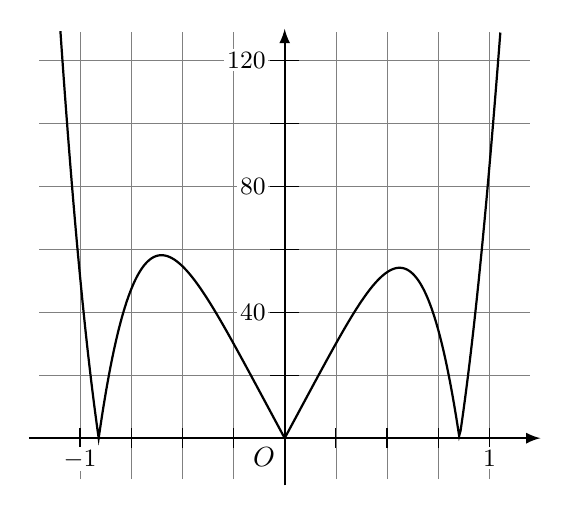
\begin{tikzpicture}[xscale=2.6,yscale=.04,declare function={f(\x)=abs(160*(\x^3)*sin((\x)^2 r)+2*\x*(16*(\x^4)-12)*cos((\x)^2 r)-96*\x*cos((\x)^2 r)-sin(\x r));},baseline=(current bounding box.north)]
        \draw[ystep=20,xstep=.25,style=help lines,] (-1.2,-13) grid (1.2,129);
        \draw[-latex, thick] (-1.25,0)--(1.25,0);
        \draw[-latex, thick] (0,-15)--(0,130);
        \foreach \x in {-1, -3/4, -.5, -.25, .25, .5, .75, 1}
            \draw (\x,90pt)--(\x,-90pt);
        \foreach \y in {20,40,60,80,100,120}
            \draw (2pt,\y)--(-2pt,\y);
        \foreach \x in {-1,1}
            \draw (\x,-1) node [below=.7mm,fill=white,inner sep=1pt] {\small$\x$};
        \foreach \y in {40,80,120}
            \draw (-.05,\y) node [left=.7mm,fill=white,inner sep=1pt] {\small$\y$};
        
        
        \draw[thick] plot [samples=300,domain=-1.0955:1.055] ({\x},{f(\x)});
        
        \node at (0,0) [below left] {$O$};
        
        
        
       %\draw[domain=-1.2:1.5, smooth,thick] plot (\x, {abs(160*(\x^3)*sin((\x)^2)+2*\x*(16*(\x^4)-12)*cos((\x)^2)-96*\x*cos((\x)^2)-sin(\x))});
    \end{tikzpicture}
    \end{center}
    \end{minipage}

    \vspace{\stretch{1}}
    
    \question The Taylor Series about $x=3$ for a certain function $f$ converges to $f(x)$ for all $x$ in the interval of convergence. The $n$th derivative of $f$ at $x=3$ is given by 
    \[\displaystyle f^{(n)}(3)\le\frac{(-1)^n \, n!}{5^n\, (n+3)}\text{for all \textit{n} and }f(3)=\frac{1}{3}.\]
    Show that $P_3(x)$ approximates $f(4)$ with an error less than $\displaystyle\frac{1}{4000}$.
    
    \vspace{\stretch{1}}


\end{questions}


\newpage
